% ============================================================
% CHAPITRE 5 : EVALUATION
% CRISP-DM - PHASE 5 (Evaluation)
% Structure canonique :
%   5.1 Evaluation des resultats au regard des objectifs metier
%   5.2 Revue du processus
%   5.3 Determination des etapes suivantes
%
% Figures : docs/rapport/img/fig_*.png  (generees par figures.py)
% Sources chiffrees : evals/results/*.json et REPORT.md
% ============================================================

\chapter{Évaluation}
\label{chap:evaluation}
\minitocsection
\newpage

% ------------------------------------------------------------
\section*{Introduction}
\addcontentsline{toc}{section}{Introduction}
% ------------------------------------------------------------

Le chapitre précédent a construit les modèles et l'architecture qui les met en œuvre, et a laissé ouverte une question : parmi les techniques retenues en concurrence pour les objectifs OD-1 et OD-3, laquelle l'emporte ? Le présent chapitre conduit la cinquième phase de CRISP-DM et y répond, mais son ambition dépasse ce départage. Il confronte l'ensemble des résultats obtenus aux critères de succès fixés au chapitre~\ref{chap:comprehension-metier}, techniques d'abord, métier ensuite.

Une règle a été tenue sans exception dans ce rapport et conditionne la crédibilité de tout ce qui suit : \textbf{aucun critère de succès n'a été modifié après l'obtention des résultats}. Les seuils du tableau~\ref{tab:criteres-succes-chap2} ont été fixés au chapitre~\ref{chap:comprehension-metier}, avant toute modélisation, et sont repris ici tels quels. Cette discipline a un coût : elle conduit à devoir reconnaître, en section~\ref{sec:bilan}, que deux objectifs ne sont pas pleinement atteints. Ce coût est assumé. Un chapitre d'évaluation dont tous les seuils sont franchis est plus souvent le signe de seuils ajustés après coup que celui d'un système exceptionnel.

Le chapitre présente d'abord le protocole d'évaluation (section~\ref{sec:protocole}), puis les résultats par famille : modèles de prévision (section~\ref{sec:eval-prevision}), décisions de stock (section~\ref{sec:eval-stock}), recommandations générées et chaîne documentaire (section~\ref{sec:eval-reco}), contrôle de conformité (section~\ref{sec:eval-conformite}), retour humain en exploitation (section~\ref{sec:eval-humain}), exigences non fonctionnelles (section~\ref{sec:eval-nfr}). La section~\ref{sec:revue-processus} conduit la revue du processus, tâche que CRISP-DM place explicitement dans cette phase et qui est le plus souvent escamotée. La section~\ref{sec:bilan} dresse le bilan d'atteinte des objectifs et énonce la décision de fin de phase.

% ------------------------------------------------------------
\section{Protocole d'évaluation}
\label{sec:protocole}
% ------------------------------------------------------------

\subsection{Niveaux d'évaluation}

Les huit objectifs analytiques ne se mesurent pas de la même façon. Trois niveaux d'évaluation ont été mis en place, chacun adapté à une nature de sortie.

Le \textbf{premier niveau} concerne les sorties numériques -- prévisions, quantités, scores. Il s'évalue par des métriques d'erreur calculées sous le protocole de rétro-test à origine glissante défini au chapitre~\ref{chap:donnees}, avec comparaison systématique à une référence naïve.

Le \textbf{deuxième niveau} concerne les sorties textuelles -- recommandations, messages de coaching, justifications. Il combine des contrôles déterministes, vérifiant des propriétés objectivement décidables, et une évaluation par juge automatique notant des critères qualitatifs sur une grille fermée \cite{zheng2023judge}.

Le \textbf{troisième niveau} est le retour humain en exploitation réelle : l'acceptation ou le refus des propositions par le responsable de point de vente. C'est le seul niveau qui mesure la valeur métier ; les deux premiers ne mesurent que la qualité technique.

\subsection{Bancs d'évaluation}

Six bancs d'évaluation ont été construits et sont rejouables. Le tableau~\ref{tab:bancs-chap5} en donne la composition.

\begingroup
\setlength{\tabcolsep}{3pt}
\renewcommand{\arraystretch}{1.15}
\small

\begin{longtable}{|P{3.1cm}|P{1.5cm}|P{4.3cm}|P{4.6cm}|}
\hline
\rowcolor{red!75}
\textcolor{white}{\textbf{Banc}} &
\textcolor{white}{\textbf{Objectif}} &
\textcolor{white}{\textbf{Jeu de test}} &
\textcolor{white}{\textbf{Nature de la mesure}} \\
\hline
\endhead
\hline
\endfoot
\hline
\endlastfoot
Rétro-test de prévision du chiffre d'affaires & OD-1 & 151 points de vente, 97 927 observations jour-boutique, 6 plis de 28 jours & Métriques d'erreur, comparaison de 5 méthodes \\
\hline
Contrôle de conformité & OD-8 & 30 cas adversariaux couvrant les 7 règles & Exactitude, précision et rappel par règle \\
\hline
Recherche documentaire & OD-7 & Jeu de référence annoté & Propriétés de recherche et métriques de fidélité \\
\hline
Coach de bout en bout & OD-6, OD-7 & 20 questions posées à l'interface réelle & Contrôles déterministes et juge automatique \\
\hline
Recommandations de stock & OD-5 & 15 cas synthétiques couvrant les 4 actions, plus un échantillon réel & Juge automatique sur 6 critères \\
\hline
Comparaison de modèles de langage & transverse & 10 questions, 2 passages, contexte figé & Score composite qualité, fiabilité, latence, coût \\
\hline
\caption{Bancs d'évaluation, objectifs couverts et nature de la mesure}
\label{tab:bancs-chap5}
\end{longtable}
\endgroup

\subsection{Précautions méthodologiques}

Quatre précautions ont été prises, dont l'absence aurait invalidé les conclusions.

L'\textbf{absence de fuite de données} est garantie par le découpage chronologique strict décrit au chapitre~\ref{chap:donnees} et par la règle d'antériorité appliquée à toute variable construite.

La \textbf{comparaison à une référence naïve} est systématique : aucun modèle n'est déclaré bon dans l'absolu, seulement meilleur ou moins bon qu'une méthode triviale.

L'\textbf{exclusion du modèle évalué du rôle de juge} est appliquée sur tous les bancs qualitatifs. Un modèle qui s'évalue lui-même se surnote, biais bien documenté et facile à éviter.

La \textbf{comparaison appariée} est imposée sur le banc de comparaison de modèles : les scores ne sont calculés que sur les questions traitées par tous les modèles. Sans cette précaution, un modèle ayant échoué sur les questions difficiles serait noté sur un sous-ensemble plus favorable et paraîtrait meilleur qu'il n'est.

% ------------------------------------------------------------
\section{Évaluation des modèles de prévision}
\label{sec:eval-prevision}
% ------------------------------------------------------------

\subsection{Prévision du chiffre d'affaires}

Le rétro-test porte sur cent cinquante et un points de vente et 97 927 observations jour-boutique, sur la période d'octobre 2024 à juillet 2026. Six plis successifs de vingt-huit jours ont été constitués selon le protocole à origine expansive, la fenêtre de test s'étendant du 12 février au 30 juillet 2026, soit 24 681 prévisions évaluées par méthode. Cinq méthodes ont été mises en concurrence. Le tableau~\ref{tab:backtest-chap5} présente les résultats agrégés.

\begingroup
\setlength{\tabcolsep}{3pt}
\renewcommand{\arraystretch}{1.15}
\small

\begin{longtable}{|P{4.4cm}|P{1.9cm}|P{1.9cm}|P{1.9cm}|P{1.6cm}|P{1.5cm}|}
\hline
\rowcolor{red!75}
\textcolor{white}{\textbf{Méthode}} &
\textcolor{white}{\textbf{WAPE \%}} &
\textcolor{white}{\textbf{MAE}} &
\textcolor{white}{\textbf{RMSE}} &
\textcolor{white}{\textbf{MASE}} &
\textcolor{white}{\textbf{Biais \%}} \\
\hline
\endhead
\hline
\endfoot
\hline
\endlastfoot
Modèle appris global & \textbf{33{,}38} & \textbf{167{,}46} & \textbf{290{,}22} & \textbf{0{,}55} & \textbf{-0{,}04} \\
\hline
Moyenne mobile 28 jours & 43{,}55 & 218{,}47 & 352{,}75 & 0{,}72 & 0{,}47 \\
\hline
Lissage exponentiel saisonnier & 46{,}30 & 232{,}27 & 393{,}91 & 0{,}76 & 3{,}12 \\
\hline
Moyenne mobile 7 jours & 46{,}49 & 233{,}22 & 389{,}12 & 0{,}77 & 2{,}76 \\
\hline
Référence naïve saisonnière & 60{,}73 & 304{,}63 & 620{,}46 & 1{,}00 & 2{,}12 \\
\hline
\caption{Rétro-test de la prévision du chiffre d'affaires journalier : 6 plis, 24 681 prévisions par méthode}
\label{tab:backtest-chap5}
\end{longtable}
\endgroup

La lecture de ce tableau appelle quatre commentaires.

\textbf{Le modèle appris global l'emporte nettement}, avec une erreur absolue pondérée de 33,38 \% contre 46,30 \% pour le moteur statistique, soit une réduction de 27,9 \% de l'erreur relative. Le critère de succès d'OD-1 -- erreur inférieure à celle d'une référence naïve, sur mesure comparative documentée -- est donc satisfait, et le départage laissé ouvert au chapitre~\ref{chap:modelisation} est tranché.

\textbf{Toutes les méthodes battent la référence naïve}, leur erreur relative à la référence étant inférieure à un. Ce constat, qui peut sembler trivial, ne l'est pas : sur des séries fortement bruitées, il n'est pas rare qu'un modèle sophistiqué soit battu par la persistance saisonnière. La valeur de 0,55 obtenue par le modèle global signifie qu'il divise par près de deux l'erreur de la méthode triviale.

\textbf{Le biais du modèle global est quasi nul} (-0,04 \%), là où toutes les autres méthodes surestiment systématiquement, jusqu'à 3,12 \% pour le lissage exponentiel. Cette propriété est importante en exploitation : un biais positif systématique conduirait le système à annoncer chaque jour au conseiller un objectif de fin de journée plus favorable que la réalité, ce qui détruirait sa crédibilité en quelques semaines.

\textbf{La supériorité du modèle global n'est pas uniforme dans le temps.} Le tableau~\ref{tab:plis-chap5} présente le détail par pli.

\begingroup
\setlength{\tabcolsep}{3pt}
\renewcommand{\arraystretch}{1.15}
\small

\begin{longtable}{|P{0.9cm}|P{3.4cm}|P{1.7cm}|P{2.0cm}|P{2.0cm}|P{2.4cm}|}
\hline
\rowcolor{red!75}
\textcolor{white}{\textbf{Pli}} &
\textcolor{white}{\textbf{Fenêtre de test}} &
\textcolor{white}{\textbf{Lignes}} &
\textcolor{white}{\textbf{Modèle global}} &
\textcolor{white}{\textbf{Lissage exp.}} &
\textcolor{white}{\textbf{Réf. naïve}} \\
\hline
\endhead
\hline
\endfoot
\hline
\endlastfoot
1 & 12/02 -- 11/03/2026 & 4 164 & \textbf{22{,}14} & 42{,}86 & 57{,}94 \\
\hline
2 & 12/03 -- 09/04/2026 & 4 155 & \textbf{22{,}16} & 42{,}65 & 55{,}18 \\
\hline
3 & 10/04 -- 07/05/2026 & 4 102 & \textbf{38{,}74} & 47{,}65 & 61{,}10 \\
\hline
4 & 08/05 -- 04/06/2026 & 3 982 & \textbf{37{,}94} & 48{,}33 & 61{,}56 \\
\hline
5 & 05/06 -- 02/07/2026 & 4 132 & \textbf{34{,}97} & 46{,}60 & 62{,}92 \\
\hline
6 & 03/07 -- 30/07/2026 & 4 146 & \textbf{40{,}93} & 48{,}67 & 64{,}17 \\
\hline
\caption{Erreur absolue pondérée par pli, en pourcentage}
\label{tab:plis-chap5}
\end{longtable}
\endgroup

L'erreur du modèle global passe de 22,1 \% sur les deux premiers plis à près de 41 \% sur le dernier. Cette dégradation est le résultat le plus instructif du banc et mérite d'être interprété honnêtement plutôt que passé sous silence. Deux explications sont plausibles et non exclusives. La première est une \textbf{dérive du modèle} : entraîné une fois, il s'éloigne progressivement des conditions courantes, ce qui est le comportement attendu et justifie la boucle de mesure quotidienne prévue au chapitre~\ref{chap:modelisation}. La seconde est un \textbf{changement de régime} sur la période estivale, où la fréquentation des points de vente se modifie. Le fait que la référence naïve se dégrade également sur les derniers plis -- de 57,9 \% à 64,2 \% -- plaide pour la seconde explication : la série elle-même devient plus difficile à prévoir. Départager ces deux causes exigerait un réentraînement à chaque pli, qui n'a pas été conduit ; c'est une limite de ce banc, et elle est reportée en section~\ref{sec:revue-processus}.

\subsection{Couverture par point de vente}

L'agrégat masque la dispersion. Le modèle global bat le moteur statistique sur \textbf{150 des 151 points de vente}, soit 99 \%. Le tableau~\ref{tab:boutiques-chap5} présente les cinq points de vente les moins favorables.

\begingroup
\setlength{\tabcolsep}{3pt}
\renewcommand{\arraystretch}{1.15}
\small

\begin{longtable}{|P{2.5cm}|P{2.8cm}|P{2.6cm}|P{3.0cm}|P{2.3cm}|}
\hline
\rowcolor{red!75}
\textcolor{white}{\textbf{Point de vente}} &
\textcolor{white}{\textbf{CA moyen}} &
\textcolor{white}{\textbf{Modèle global}} &
\textcolor{white}{\textbf{Lissage exp.}} &
\textcolor{white}{\textbf{Écart}} \\
\hline
\endhead
\hline
\endfoot
\hline
\endlastfoot
I14 & 1 809{,}4 & 52{,}85 & 33{,}22 & \textbf{+19{,}63} \\
\hline
M10 & 3 473{,}9 & 11{,}89 & 13{,}56 & -1{,}67 \\
\hline
I60 & 710{,}6 & 24{,}98 & 28{,}09 & -3{,}11 \\
\hline
S20 & 549{,}6 & 25{,}46 & 28{,}63 & -3{,}17 \\
\hline
S47 & 1 642{,}4 & 22{,}73 & 26{,}22 & -3{,}49 \\
\hline
\caption{Points de vente les moins favorables au modèle global (erreur absolue pondérée, \%)}
\label{tab:boutiques-chap5}
\end{longtable}
\endgroup

Un seul point de vente, I14, met le modèle global en échec, avec une erreur de 52,9 \% contre 33,2 \% pour le moteur statistique. Ce cas isolé est précisément ce qui justifie la conception en cascade retenue au chapitre~\ref{chap:modelisation} : le moteur statistique n'est pas un vestige mais un recours, et il reste disponible pour les points de vente où le modèle appris est moins performant. Un système qui aurait remplacé purement et simplement le premier par le second aurait dégradé la prévision de ce point de vente sans possibilité de retour.

\subsection{Prévision de la demande par référence}

L'objectif OD-3 dispose d'une chaîne de mesure en exploitation plutôt que d'un rétro-test unique : chaque jour, la prévision de la veille -- de base et corrigée -- est confrontée aux ventes réellement observées et l'erreur est enregistrée. Ce dispositif, décrit au chapitre~\ref{chap:modelisation}, présente l'avantage de mesurer la performance dans les conditions réelles d'exploitation plutôt qu'en laboratoire.

Le modèle de correction contextuelle a été départagé de son principal concurrent lors de la phase de construction, sur la table d'entraînement constituée au chapitre~\ref{chap:donnees}. Le gradient boosté l'a emporté et a été retenu.

Un incident de réentraînement mérite d'être rapporté, car il illustre la valeur du dispositif de mesure. Une version du modèle publiée initialement présentait une erreur voisine de 100 \%, c'est-à-dire une prévision sans aucune valeur informative. Le défaut ne provenait pas de la méthode mais de la version du modèle effectivement chargée en production, qui n'était pas celle entraînée sur la table de variables corrigée. Le réentraînement sur la table à jour a ramené l'erreur à un ordre de grandeur inférieur à 10 \%. Sans mesure quotidienne, ce défaut serait resté invisible : le système produisait des prévisions plausibles, simplement fausses. C'est l'argument le plus concret en faveur de l'instrumentation d'un modèle en production.

% ------------------------------------------------------------
\section{Évaluation des décisions de stock}
\label{sec:eval-stock}
% ------------------------------------------------------------

\subsection{Cohérence de la classification du risque}

Le critère de succès d'OD-4 est une propriété de cohérence, non une métrique d'erreur : aucune référence à stock nul ne doit être classée autrement qu'en risque critique. Cette propriété a été vérifiée par test automatisé sur l'ensemble des couples référence et point de vente évalués, ainsi que sur un jeu de cas limites construit spécifiquement : stock nul, stock nul avec commande en transit, couverture juste inférieure au délai, couverture juste supérieure, seuils de gestion contradictoires avec le calcul.

La propriété est vérifiée sans exception. La règle de sévérité maximale entre les deux couches de classification garantit par construction qu'un seuil de gestion ne peut jamais atténuer un diagnostic de rupture produit par le calcul, ni l'inverse. Le critère de succès d'OD-4 est atteint.

\subsection{Qualité des recommandations de réapprovisionnement}

La justification produite par l'agent Décision a été évaluée par juge automatique sur quinze cas synthétiques couvrant les quatre actions possibles, puis sur un échantillon de cas réels. Le tableau~\ref{tab:decision-chap5} présente les résultats.

\begingroup
\setlength{\tabcolsep}{3pt}
\renewcommand{\arraystretch}{1.15}
\small

\begin{longtable}{|P{3.4cm}|P{3.1cm}|P{3.1cm}|P{4.0cm}|}
\hline
\rowcolor{red!75}
\textcolor{white}{\textbf{Critère (0--5)}} &
\textcolor{white}{\textbf{Cas synthétiques}} &
\textcolor{white}{\textbf{Échantillon réel}} &
\textcolor{white}{\textbf{Lecture}} \\
\hline
\endhead
\hline
\endfoot
\hline
\endlastfoot
Clarté & 5{,}00 & 5{,}00 & Formulation compréhensible sans expertise \\
\hline
Cohérence & 4{,}80 & 5{,}00 & Décision compatible avec les chiffres cités \\
\hline
Complétude & 4{,}87 & 4{,}00 & Tous les éléments de décision présents \\
\hline
Actionnabilité & 4{,}93 & 5{,}00 & Le destinataire sait quoi faire \\
\hline
Richesse & 4{,}73 & 4{,}00 & Justification argumentée, non templatée \\
\hline
Ancrage & 4{,}20 & 5{,}00 & Chiffres traçables au contexte fourni \\
\hline
\rowcolor{gray!12}
\textbf{Moyenne} & \textbf{4{,}76} & \textbf{5{,}00} & 15 cas / 3 cas \\
\hline
\caption{Évaluation par juge automatique des justifications de l'agent Décision}
\label{tab:decision-chap5}
\end{longtable}
\endgroup

Ces valeurs sont élevées, et c'est précisément ce qui impose la prudence dans leur interprétation. Trois réserves doivent être formulées.

La première tient à la \textbf{taille des échantillons} : quinze cas synthétiques et trois cas réels. L'échantillon réel, en particulier, ne peut être lu que comme un instantané et non comme un seuil de non-régression.

La deuxième tient à la \textbf{validation du juge lui-même}. Trois contrôles avaient été prévus pour établir que le juge discrimine effectivement : vérifier qu'il note plus bas une justification produite par un gabarit rigide que par le modèle, vérifier qu'il détecte un chiffre volontairement corrompu, et vérifier qu'il attribue la même note au même texte rejoué. \textbf{Ces trois contrôles n'ont pas été exécutés.} Sans eux, rien n'établit qu'un juge notant tout à 4,8 ne noterait pas également 4,8 une justification médiocre. Les valeurs du tableau~\ref{tab:decision-chap5} doivent donc être lues comme indicatives, et non comme une mesure établie. Cette lacune est reportée en section~\ref{sec:revue-processus}.

La troisième tient à l'\textbf{écart entre banc et exploitation}, qui sera constaté en section~\ref{sec:eval-humain} et qui est le résultat le plus significatif de ce chapitre.

\subsection{Sensibilité au paramétrage logistique}

Le chapitre~\ref{chap:donnees} avait identifié que les paramètres logistiques -- délais, coûts de possession et de passation, quantités minimales -- sont pour une large part laissés à leur valeur par défaut, et avait annoncé que l'effet en serait mesuré séparément. Ce point est central pour l'honnêteté de l'évaluation d'OD-5.

La méthode de calcul est vérifiée : les formules du chapitre~\ref{chap:modelisation} sont implémentées conformément à leur énoncé et testées unitairement, y compris sur les cas dégénérés -- coût unitaire nul, demande nulle, écart-type nul -- où des valeurs de repli documentées s'appliquent. La \textbf{justesse de la méthode} est donc établie.

La \textbf{justesse des valeurs produites} ne l'est pas, et ne peut pas l'être. La quantité économique de commande varie comme la racine carrée du rapport entre coût de passation et coût de possession ; lorsque ces deux coûts sont des valeurs par défaut, la quantité obtenue est un ordre de grandeur défendable, non une valeur optimale. Il en va de même du stock de sécurité, dont le terme dominant dépend de l'écart-type du délai fournisseur, rarement renseigné.

Cette limite ne relève pas de la modélisation mais de la donnée. La présenter comme une faiblesse du système serait inexact ; la passer sous silence le serait davantage. Elle est donc énoncée comme une condition de déploiement en section~\ref{sec:bilan} : la valeur des quantités recommandées progressera avec la qualité du paramétrage, indépendamment de toute amélioration des modèles.

% ------------------------------------------------------------
\section{Évaluation des recommandations générées et de la chaîne documentaire}
\label{sec:eval-reco}
% ------------------------------------------------------------

\subsection{Chaîne de recherche documentaire}

L'objectif OD-7 a été évalué sur deux registres complémentaires. Le premier mesure les \textbf{propriétés de la recherche} sur un jeu de référence annoté ; le second mesure la \textbf{fidélité de la génération ancrée} par des métriques dédiées aux systèmes de génération augmentée par la recherche \cite{es2024ragas}. Le tableau~\ref{tab:rag-chap5} présente les deux.

\begingroup
\setlength{\tabcolsep}{3pt}
\renewcommand{\arraystretch}{1.15}
\small

\begin{longtable}{|P{4.6cm}|P{2.2cm}|P{6.6cm}|}
\hline
\rowcolor{red!75}
\textcolor{white}{\textbf{Métrique}} &
\textcolor{white}{\textbf{Valeur}} &
\textcolor{white}{\textbf{Lecture}} \\
\hline
\endhead
\hline
\endfoot
\hline
\endlastfoot
\multicolumn{3}{|l|}{\textit{Propriétés de recherche (jeu de référence annoté)}} \\
\hline
Présence dans les 3 premiers & 100 \% & Le bon domaine documentaire est toujours remonté \\
\hline
Rang réciproque moyen & 0{,}955 & Le bon document est presque toujours en tête \\
\hline
Rappel de contenu & 100 \% & Le contenu attendu est effectivement retrouvé \\
\hline
Pureté & 100 \% & Aucun contenu interdit n'est remonté \\
\hline
Abstention & 100 \% & Le système sait déclarer qu'il n'a rien de pertinent \\
\hline
\multicolumn{3}{|l|}{\textit{Fidélité de la génération ancrée (8 cas)}} \\
\hline
Fidélité aux sources & 0{,}81 & La réponse n'affirme rien hors des extraits fournis \\
\hline
Précision du contexte & 0{,}75 & Les extraits remontés sont utiles à la réponse \\
\hline
Pertinence de la réponse & 0{,}544 & La réponse traite effectivement la question posée \\
\hline
Couverture du contexte & 0{,}248 & Les extraits couvrent l'information de référence \\
\hline
\caption{Évaluation de la chaîne de recherche documentaire}
\label{tab:rag-chap5}
\end{longtable}
\endgroup

Le contraste entre les deux moitiés de ce tableau est frappant et instructif. Les propriétés de recherche sont excellentes : le système retrouve ce qu'il faut, ne remonte rien d'interdit, et sait s'abstenir. La capacité d'abstention, à 100 \%, est particulièrement significative : c'est elle qui distingue une chaîne documentaire fiable d'une chaîne qui produit une réponse plausible en toute circonstance \cite{ji2023hallucination}.

Les métriques de génération ancrée sont en revanche contrastées. La fidélité aux sources, à 0,81, est satisfaisante : la réponse n'invente pas. Mais la \textbf{couverture du contexte, à 0,248, est faible} : les extraits remontés ne contiennent qu'une part de l'information nécessaire à une réponse complète. Cette faiblesse ne provient pas du mécanisme de recherche, dont les propriétés sont bonnes, mais de la \textbf{densité du corpus} : la connaissance métier disponible ne couvre pas toutes les questions du jeu de test. Le diagnostic est donc un manque de contenu et non un défaut d'algorithme, ce qui appelle un enrichissement du corpus plutôt qu'une modification de la chaîne.

Le critère de succès d'OD-7 -- chaque affirmation chiffrée rattachée à une source citée -- porte sur la fidélité et non sur la couverture ; il est satisfait. Mais la faiblesse de couverture est une limite réelle et elle est reportée au bilan.

\subsection{Coach conversationnel de bout en bout}

Le banc de bout en bout interroge l'interface réelle avec vingt questions représentatives, et évalue les réponses par contrôles déterministes puis par juge automatique. Le tableau~\ref{tab:coach-chap5} présente les résultats.

\begingroup
\setlength{\tabcolsep}{3pt}
\renewcommand{\arraystretch}{1.15}
\small

\begin{longtable}{|P{5.6cm}|P{2.6cm}|P{5.2cm}|}
\hline
\rowcolor{red!75}
\textcolor{white}{\textbf{Indicateur}} &
\textcolor{white}{\textbf{Valeur}} &
\textcolor{white}{\textbf{Commentaire}} \\
\hline
\endhead
\hline
\endfoot
\hline
\endlastfoot
Taux de réponse & 100 \% (20/20) & Aucune requête sans réponse \\
\hline
Contrôles déterministes & 84{,}6 \% & Remise interdite, fuite de consigne, refus hors sujet, langue \\
\hline
Score du juge, global & 4{,}14 / 5 & Moyenne des cinq critères \\
\hline
\quad Pertinence & 3{,}30 & Critère le plus faible \\
\hline
\quad Ancrage & 4{,}33 & Sur les cas à contexte complet \\
\hline
\quad Actionnabilité & 3{,}65 & \\
\hline
\quad Langue & 4{,}55 & \\
\hline
\quad Sécurité & 4{,}80 & Critère le plus élevé \\
\hline
Taux d'hallucination & 16{,}7 \% & Sur les 18 cas à contexte complet \\
\hline
Taux d'usage de la recherche documentaire & 0 \% & \textbf{Anomalie -- voir ci-dessous} \\
\hline
\caption{Évaluation de bout en bout de l'agent Coach sur 20 questions}
\label{tab:coach-chap5}
\end{longtable}
\endgroup

Trois observations s'imposent.

\textbf{Le profil de notation est cohérent avec la conception.} Les critères les mieux notés sont la sécurité et la langue, précisément ceux que les garde-fous et la consigne système contraignent explicitement. Les critères les moins bien notés sont la pertinence et l'actionnabilité, qui dépendent de la richesse du contexte fourni et non de contraintes formelles. Le système est donc plus fiable qu'il n'est pertinent -- ordre de priorité défendable pour un assistant destiné à un usage professionnel, mais qui borne la valeur perçue.

\textbf{Le taux d'usage de la recherche documentaire est nul}, ce qui est anormal. Sur les vingt questions, aucune réponse n'a mobilisé le corpus, alors que plusieurs s'y prêtaient. Ce résultat s'explique par l'indisponibilité de la base vectorielle lors de l'exécution du banc : le mécanisme de repli a fonctionné comme prévu -- le système a répondu au lieu d'échouer -- mais les réponses ont été produites sans l'ancrage documentaire attendu. Deux conclusions en découlent. D'une part, la robustesse conçue au chapitre~\ref{chap:modelisation} est confirmée en conditions de panne réelle. D'autre part, \textbf{les scores de ce banc mesurent le système en mode dégradé} et sous-estiment vraisemblablement ses performances nominales. Ils sont donc une borne inférieure, ce qui est une lecture honnête mais qui interdit de les présenter comme la performance du système.

\textbf{Le taux d'hallucination de 16,7 \%} est élevé et doit être énoncé sans atténuation. Il signifie qu'environ une réponse sur six contient une affirmation non dérivable du contexte fourni. Ce taux est cohérent avec l'absence d'ancrage documentaire constatée ci-dessus : privé du corpus, le modèle comble par sa mémoire paramétrique. Il constitue la principale réserve technique du système et justifie pleinement le maintien du contrôle de conformité en aval.

\subsection{Comparaison des modèles de langage}

Le choix du modèle affecté à chaque rôle, annoncé au chapitre~\ref{chap:modelisation}, s'appuie sur un banc comparatif conduit sur dix questions à contexte figé, deux passages, et un panel de juges distincts du modèle évalué. Le tableau~\ref{tab:modeles-chap5} présente les résultats.

\begingroup
\setlength{\tabcolsep}{3pt}
\renewcommand{\arraystretch}{1.15}
\small

\begin{longtable}{|P{3.9cm}|P{1.6cm}|P{1.5cm}|P{2.2cm}|P{1.6cm}|P{1.9cm}|}
\hline
\rowcolor{red!75}
\textcolor{white}{\textbf{Modèle}} &
\textcolor{white}{\textbf{Composite}} &
\textcolor{white}{\textbf{Qualité}} &
\textcolor{white}{\textbf{IC 95 \%}} &
\textcolor{white}{\textbf{Latence}} &
\textcolor{white}{\textbf{Coût rel.}} \\
\hline
\endhead
\hline
\endfoot
\hline
\endlastfoot
Mistral Small & \textbf{0{,}953} & 4{,}88 & 4{,}79 -- 4{,}97 & 1 775 ms & 0{,}078 \\
\hline
Llama 3.3 70B & 0{,}861 & 4{,}79 & 4{,}65 -- 4{,}91 & 1 357 ms & 0{,}370 \\
\hline
GPT-OSS 120B & 0{,}842 & 4{,}91 & 4{,}78 -- 5{,}00 & 1 765 ms & 0{,}327 \\
\hline
Mistral Large & 0{,}733 & 4{,}92 & 4{,}80 -- 4{,}99 & 4 545 ms & 1{,}951 \\
\hline
Nemotron (2 variantes) & 0{,}150 & --- & --- & --- & indisponibles \\
\hline
\caption{Comparaison des modèles de langage : score composite et détail}
\label{tab:modeles-chap5}
\end{longtable}
\endgroup

Le résultat le plus important de ce banc n'est pas le classement mais son \textbf{absence de significativité en qualité}. Les intervalles de confiance à 95 \% des quatre modèles disponibles se chevauchent tous : sur ce jeu de test, \textbf{aucune différence de qualité n'est statistiquement établie entre eux}. Le classement composite n'est donc pas déterminé par la qualité mais par les trois autres composantes -- fiabilité, latence et coût --, dont les écarts sont eux considérables : Mistral Large est 2,6 fois plus lent et 25 fois plus coûteux que Mistral Small pour une qualité indiscernable.

Cette conclusion, contre-intuitive, aurait été manquée par un protocole sans intervalles de confiance : le classement par qualité brute plaçait Mistral Large en tête, et aurait conduit à retenir le modèle le plus cher et le plus lent sur la foi d'un écart de 0,04 point sans signification statistique. C'est l'apport méthodologique principal de ce banc.

Deux modèles annoncés comme disponibles se sont révélés inaccessibles pendant toute la durée du banc. Leur exclusion est traitée comme un défaut de fiabilité et pénalise leur score composite, ce qui est le comportement souhaité : un modèle indisponible a une qualité opérationnelle nulle, quelle que soit sa qualité intrinsèque.

% ------------------------------------------------------------
\section{Évaluation du contrôle de conformité}
\label{sec:eval-conformite}
% ------------------------------------------------------------

Le contrôle de conformité a été évalué sur un jeu adversarial de trente cas, construit de manière à ce que chacune des sept règles soit sollicitée à la fois par des cas devant la déclencher et par des cas ne devant pas la déclencher. Cette construction est essentielle : un jeu ne contenant que des violations mesurerait la sensibilité sans mesurer la spécificité, et un contrôle bloquant tout obtiendrait un score parfait.

Le tableau~\ref{tab:guardrail-chap5} présente les résultats.

\begingroup
\setlength{\tabcolsep}{3pt}
\renewcommand{\arraystretch}{1.15}
\small

\begin{longtable}{|P{1.2cm}|P{6.1cm}|P{1.8cm}|P{1.6cm}|P{1.4cm}|}
\hline
\rowcolor{red!75}
\textcolor{white}{\textbf{Règle}} &
\textcolor{white}{\textbf{Objet du contrôle}} &
\textcolor{white}{\textbf{Précision}} &
\textcolor{white}{\textbf{Rappel}} &
\textcolor{white}{\textbf{F1}} \\
\hline
\endhead
\hline
\endfoot
\hline
\endlastfoot
G1 & Produit à stock nul & 1{,}00 & 1{,}00 & 1{,}00 \\
\hline
G2 & Rupture imminente & 1{,}00 & 1{,}00 & 1{,}00 \\
\hline
G3 & Ancrage documentaire de l'argument & 1{,}00 & 1{,}00 & 1{,}00 \\
\hline
G4 & Remise ou offre non autorisée & 1{,}00 & 1{,}00 & 1{,}00 \\
\hline
G5 & Éligibilité technique & 1{,}00 & 1{,}00 & 1{,}00 \\
\hline
G6 & Confiance insuffisante & 1{,}00 & 1{,}00 & 1{,}00 \\
\hline
G7 & Engagement financier & 1{,}00 & 1{,}00 & 1{,}00 \\
\hline
\rowcolor{gray!12}
\multicolumn{2}{|l|}{\textbf{Exactitude du statut sur 30 cas}} & \multicolumn{3}{c|}{\textbf{100 \%}} \\
\hline
\rowcolor{gray!12}
\multicolumn{2}{|l|}{\textbf{Taux de faux blocage}} & \multicolumn{3}{c|}{\textbf{0 \%}} \\
\hline
\caption{Évaluation du contrôle de conformité sur un jeu adversarial de 30 cas}
\label{tab:guardrail-chap5}
\end{longtable}
\endgroup

Le contrôle atteint une exactitude parfaite sur ce jeu, et surtout un taux de faux blocage nul : aucune recommandation légitime n'a été bloquée ni escaladée à tort. Cette seconde propriété est plus importante que la première pour l'acceptabilité du système. Un contrôle trop strict serait rapidement contourné par les utilisateurs.

Ce résultat doit cependant être interprété pour ce qu'il est. Les règles sont \textbf{déterministes} : ce sont des conditions explicites appliquées à des valeurs calculées, non un classifieur appris. Obtenir une exactitude de 100 \% sur un jeu couvrant les cas prévus est donc le comportement attendu, et non une performance remarquable. Ce que le banc établit réellement, c'est que les règles sont correctement \textbf{implémentées} et qu'elles ne se déclenchent pas à tort -- ce qui est utile mais différent d'une capacité de généralisation. Un cas non anticipé lors de la conception des règles ne sera pas détecté, quelle que soit la qualité du score obtenu ici. Cette limite est intrinsèque à l'approche par règles, assumée au chapitre~\ref{chap:modelisation} en échange de l'auditabilité du verdict.

La vérification exigée par le critère de succès d'OD-8 -- aucune diffusion contrevenant à une règle bloquante -- est satisfaite : sur l'ensemble des cycles exécutés, aucune recommandation ayant déclenché G1 ou G4 n'a été transmise à l'interface.

% ------------------------------------------------------------
\section{Évaluation par le retour humain en exploitation}
\label{sec:eval-humain}
% ------------------------------------------------------------

\subsection{Taux d'acceptation}

Le niveau d'évaluation le plus exigeant est celui du retour humain : les propositions du système sont-elles acceptées par le responsable qui doit les assumer ? Sur une période d'observation de trente jours, quatre-vingt-une décisions ont été tracées, dont trente-neuf approuvées, soit un \textbf{taux d'acceptation de 48,1 \%} et un taux de rejet de 51,9 \%.

Le critère de succès d'OD-5, fixé au chapitre~\ref{chap:comprehension-metier}, exigeait qu'une \textbf{majorité} des propositions soit approuvée. \textbf{Ce critère n'est pas atteint.} Ce constat est énoncé sans atténuation, conformément à la règle de non-révision des seuils posée en introduction.

Deux éléments doivent cependant accompagner ce constat pour qu'il soit lu correctement. Le premier est que le taux de rejet, à 51,9 \%, est \textbf{supérieur de 8,3 points à la référence des trois mois précédents} (43,6 \%), ce qui indique une dégradation et non un état stable. Le second est la répartition par boucle de décision : les propositions de bons de commande et les recommandations de réapprovisionnement présentent des volumes comparables d'approbations et de rejets, tandis que les stratégies commerciales soumises à validation sont massivement rejetées. La figure~\ref{fig:feedback-chap5} présente cette répartition.

\begin{figure}[H]
    \centering
    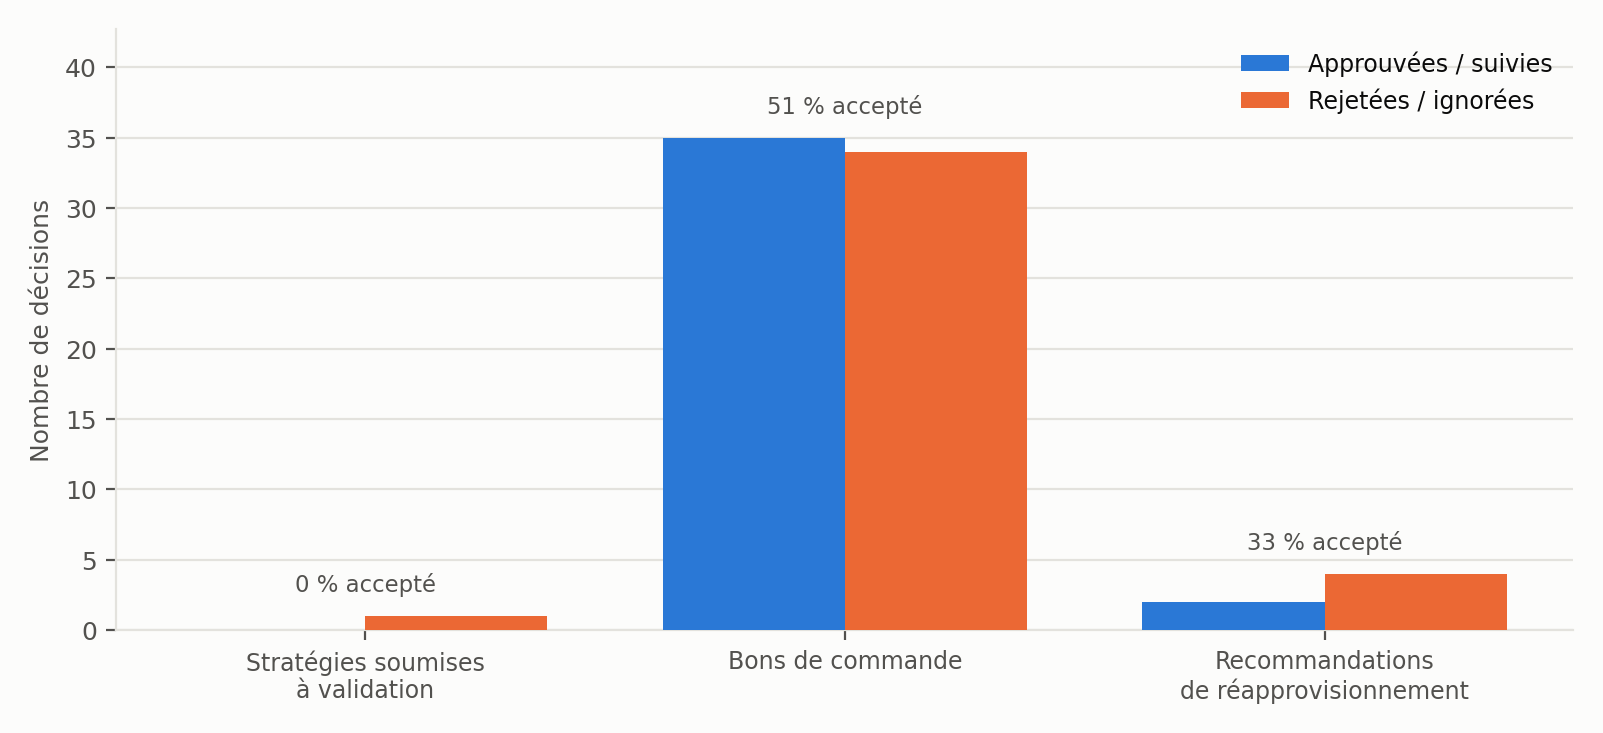
\includegraphics[width=\textwidth]{img/fig_feedback_boucles.png}
    \caption{Décisions approuvées et rejetées par boucle de décision, sur 30 jours}
    \label{fig:feedback-chap5}
\end{figure}

Le diagnostic est donc \textbf{différencié} : le domaine des stocks est proche de l'équilibre, le domaine des stratégies commerciales est en échec. Traiter ces deux situations par une moyenne unique masquerait l'information utile.

\subsection{Qualité mesurée en exploitation}

Un juge automatique fonctionne également en continu sur les productions réelles du système, indépendamment des bancs hors ligne. Le tableau~\ref{tab:qualite-live-chap5} présente ses résultats sur la même période.

\begingroup
\setlength{\tabcolsep}{3pt}
\renewcommand{\arraystretch}{1.15}
\small

\begin{longtable}{|P{4.3cm}|P{2.6cm}|P{2.6cm}|P{3.4cm}|}
\hline
\rowcolor{red!75}
\textcolor{white}{\textbf{Critère}} &
\textcolor{white}{\textbf{Recos stock}} &
\textcolor{white}{\textbf{Stratégies vente}} &
\textcolor{white}{\textbf{Écart au banc}} \\
\hline
\endhead
\hline
\endfoot
\hline
\endlastfoot
Clarté / Pertinence & 4{,}35 & 2{,}96 & --- \\
\hline
Cohérence / Ancrage & 3{,}43 & --- & --- \\
\hline
Complétude / Actionnabilité & 3{,}74 & 2{,}75 & --- \\
\hline
Actionnabilité / Langue & 4{,}70 & 3{,}54 & --- \\
\hline
Richesse / Sécurité & 3{,}52 & 4{,}75 & --- \\
\hline
Ancrage & 5{,}00 & --- & --- \\
\hline
\rowcolor{gray!12}
\textbf{Moyenne} & \textbf{3{,}58 / 5} & \textbf{3{,}18 / 5} & \textbf{-1{,}18 pt} \\
\hline
\multicolumn{4}{|l|}{\textit{Score global toutes productions confondues : 3{,}38 / 5 sur 47 recommandations notées}} \\
\hline
\caption{Qualité mesurée en exploitation par juge automatique, sur 30 jours}
\label{tab:qualite-live-chap5}
\end{longtable}
\endgroup

C'est ici que se situe le \textbf{résultat le plus significatif de ce chapitre}. Le score de qualité mesuré en exploitation, 3,38 sur 5, est très inférieur à celui obtenu sur les bancs hors ligne : 4,76 pour les recommandations de stock sur cas synthétiques, 4,14 pour le coach sur questions préparées. L'écart atteint 1,18 point sur le seul domaine des stocks, où la comparaison est directe.

Cet écart n'est pas une anomalie de mesure : il est la manifestation d'un phénomène bien connu et rarement rapporté. Les \textbf{cas de banc sont propres} : le contexte y est complet, la situation caractéristique, l'énoncé bien formé. Les \textbf{cas réels sont sales} : contexte partiel, situations ambiguës, références mal paramétrées, données manquantes. Un système évalué uniquement hors ligne paraît donc systématiquement meilleur qu'il n'est.

La conséquence méthodologique est directe et vaut d'être énoncée en soutenance : \textbf{un banc hors ligne mesure une borne supérieure, pas une performance}. C'est la raison pour laquelle le troisième niveau d'évaluation -- le retour humain en exploitation -- a été mis en place et est traité ici comme le juge de dernier ressort, et non comme un complément décoratif des mesures automatiques.

\subsection{Fiabilité des sources en exploitation}

Le même dispositif mesure en continu la fiabilité de la chaîne documentaire sur les cas réels : fidélité aux sources 81 \%, précision du contexte 75 \%, pertinence de la réponse 54 \%, couverture du contexte 25 \%. Ces valeurs confirment en exploitation le diagnostic établi hors ligne en section~\ref{sec:eval-reco} : le mécanisme de recherche fonctionne, le corpus manque de densité. La convergence des deux mesures, obtenues par des voies indépendantes, renforce la confiance dans ce diagnostic.

% ------------------------------------------------------------
\section{Évaluation des exigences non fonctionnelles}
\label{sec:eval-nfr}
% ------------------------------------------------------------

Le tableau~\ref{tab:nfr-chap5} confronte chaque exigence non fonctionnelle du chapitre~\ref{chap:comprehension-metier} à sa mesure.

\begingroup
\setlength{\tabcolsep}{3pt}
\renewcommand{\arraystretch}{1.15}
\small

\begin{longtable}{|P{1.2cm}|P{3.5cm}|P{4.2cm}|P{2.5cm}|P{2.0cm}|}
\hline
\rowcolor{red!75}
\textcolor{white}{\textbf{Réf.}} &
\textcolor{white}{\textbf{Exigence}} &
\textcolor{white}{\textbf{Mesure}} &
\textcolor{white}{\textbf{Cible}} &
\textcolor{white}{\textbf{Verdict}} \\
\hline
\endhead
\hline
\endfoot
\hline
\endlastfoot
BNF-1 & Latence du diagnostic analytique & Moteur de séries temporelles $<$ 1 s & Temps réel & Atteint \\
\hline
BNF-1 & Latence conversationnelle & Médiane 6{,}4 s ; 95\textsuperscript{e} centile 41{,}7 s & Réponse progressive & Partiel \\
\hline
BNF-2 & Disponibilité en cas de panne de fournisseur & Taux de réponse 100 \% avec base vectorielle indisponible & Aucune interruption & Atteint \\
\hline
BNF-3 & Cloisonnement par rôle et par point de vente & Vérifié par tests d'accès et parcours applicatif & Étanche & Atteint \\
\hline
BNF-4 & Traçabilité des productions & 81 décisions tracées sur 30 jours, chaîne causale complète & Traçabilité intégrale & Atteint \\
\hline
BNF-5 & Robustesse de la chaîne de génération & Cascade éprouvée en conditions de panne réelle & Dégradation, non interruption & Atteint \\
\hline
BNF-6 & Ergonomie mobile & Parcours conseiller vérifié sur format téléphone & Utilisable & Atteint \\
\hline
BNF-7 & Maintenabilité & Schéma versionné, tests unitaires et de bout en bout, intégration continue & Reprise possible & Atteint \\
\hline
\caption{Évaluation des exigences non fonctionnelles}
\label{tab:nfr-chap5}
\end{longtable}
\endgroup

Une seule exigence n'est que partiellement satisfaite : la latence conversationnelle. La médiane de 6,4 secondes est acceptable dans un contexte où la réponse s'affiche progressivement, l'utilisateur voyant le texte se construire. Le 95\textsuperscript{e} centile de 41,7 secondes ne l'est pas : une réponse sur vingt fait attendre le conseiller près de trois quarts de minute, ce qui est incompatible avec un usage au comptoir. La cause en est identifiée -- l'enchaînement des replis de la cascade lorsque le fournisseur primaire est saturé -- et le levier de correction également : abaisser le budget de latence par niveau, au prix d'un basculement plus fréquent vers un modèle de repli. Cet arbitrage n'a pas été tranché et figure parmi les évolutions proposées.

% ------------------------------------------------------------
\section{Revue du processus}
\label{sec:revue-processus}
% ------------------------------------------------------------

CRISP-DM prévoit explicitement, au sein de la phase d'évaluation, une revue du processus lui-même, distincte de l'évaluation des résultats. Cette tâche est fréquemment omise ; elle est conduite ici.

\subsection{Ce qui a été fait correctement}

Le \textbf{protocole de découpage temporel} a été défini avant toute modélisation et respecté sans exception, y compris dans le calcul des variables construites. Aucun résultat de ce chapitre n'est entaché de fuite de données.

La \textbf{comparaison systématique à une référence naïve} a été maintenue sur tous les bancs quantitatifs, ce qui a permis d'établir que la valeur ajoutée des modèles est réelle et de la chiffrer.

Le recours aux \textbf{intervalles de confiance} sur le banc comparatif de modèles a évité une erreur de sélection coûteuse, comme montré en section~\ref{sec:eval-reco}.

La mise en place d'une \textbf{mesure en exploitation}, indépendante des bancs hors ligne, a révélé un écart de plus d'un point de qualité qu'aucune évaluation hors ligne n'aurait mis au jour.

\subsection{Ce qui a été négligé}

Trois lacunes doivent être reconnues.

La \textbf{validation du juge automatique n'a pas été menée à son terme}. Les trois contrôles prévus -- discrimination sur gabarit, détection de chiffre corrompu, déterminisme sur texte rejoué -- n'ont pas été exécutés. En conséquence, les scores des tableaux~\ref{tab:decision-chap5} et~\ref{tab:coach-chap5} doivent être lus comme indicatifs. C'est la lacune la plus sérieuse de ce chapitre, car elle affecte la valeur probante de l'ensemble des mesures qualitatives.

Le \textbf{banc de prévision n'a pas été rejoué avec réentraînement à chaque pli}. Il ne permet donc pas de distinguer la dérive du modèle du changement de régime de la série, alors que cette distinction commande la fréquence de réentraînement à retenir en exploitation.

Les \textbf{tailles d'échantillon des bancs qualitatifs sont faibles} : vingt questions pour le coach, quinze cas pour l'agent Décision, huit cas pour la fidélité documentaire, dix questions pour la comparaison de modèles. Ces volumes autorisent des constats d'ordre de grandeur, non des conclusions fines. Toute différence inférieure à quelques dixièmes de point sur ces bancs doit être considérée comme non significative.

\subsection{Ce qu'il faudrait refaire}

Trois actions sont identifiées, par ordre de priorité décroissante : exécuter les trois contrôles de validation du juge avant toute publication ultérieure de scores qualitatifs ; rejouer le rétro-test de prévision avec réentraînement par pli ; élargir le corpus documentaire, dont la faible couverture est le facteur limitant commun à la pertinence du coach et à la qualité de la génération ancrée.

% ------------------------------------------------------------
\section{Bilan d'atteinte des objectifs}
\label{sec:bilan}
% ------------------------------------------------------------

\subsection{Objectifs analytiques}

Le tableau~\ref{tab:bilan-od-chap5} confronte chaque objectif analytique au critère fixé au chapitre~\ref{chap:comprehension-metier}.

\begingroup
\setlength{\tabcolsep}{3pt}
\renewcommand{\arraystretch}{1.15}
\small

\begin{longtable}{|P{1.1cm}|P{4.2cm}|P{4.6cm}|P{3.3cm}|}
\hline
\rowcolor{red!75}
\textcolor{white}{\textbf{Réf.}} &
\textcolor{white}{\textbf{Critère fixé au ch. 2}} &
\textcolor{white}{\textbf{Résultat obtenu}} &
\textcolor{white}{\textbf{Verdict}} \\
\hline
\endhead
\hline
\endfoot
\hline
\endlastfoot
OD-1 & Erreur inférieure à la référence naïve, sur mesure comparative documentée & 33{,}4 \% contre 60{,}7 \% ; MASE 0{,}55 ; 5 méthodes comparées sur 6 plis & \textbf{Atteint} \\
\hline
OD-2 & Toute heure au-delà du seuil signalée, sans saturation d'alertes & Écart normalisé par heure, statuts cohérents, pas de saturation observée & \textbf{Atteint} \\
\hline
OD-3 & Amélioration mesurable par rapport à la prévision sans correction & Correction contextuelle retenue sur banc comparatif ; mesure quotidienne en exploitation & \textbf{Atteint} \\
\hline
OD-4 & Aucune référence à stock nul classée autrement qu'en rupture & Propriété vérifiée sans exception, y compris sur les cas limites & \textbf{Atteint} \\
\hline
OD-5 & Majorité des propositions approuvées, motifs analysés & 48{,}1 \% d'acceptation sur 81 décisions ; motifs collectés et analysés & \textbf{Non atteint} \\
\hline
OD-6 & Aucun produit indisponible dans la liste proposée & Garanti par la règle G1, 0 \% de faux blocage & \textbf{Atteint} \\
\hline
OD-7 & Chaque affirmation chiffrée rattachée à une source citée & Fidélité 0{,}81 ; abstention 100 \% ; \textbf{couverture du corpus faible (0{,}248)} & \textbf{Partiel} \\
\hline
OD-8 & Score conforme au seuil ; aucune diffusion contrevenant à une règle bloquante & Exactitude 100 \%, faux blocage 0 \% ; qualité en exploitation 3{,}38/5 & \textbf{Partiel} \\
\hline
\caption{Bilan d'atteinte des objectifs analytiques}
\label{tab:bilan-od-chap5}
\end{longtable}
\endgroup

Cinq objectifs sur huit sont pleinement atteints, deux le sont partiellement, un ne l'est pas.

L'objectif \textbf{OD-5 n'est pas atteint} : le taux d'acceptation de 48,1 \% est en deçà de la majorité exigée. L'analyse des motifs de rejet montre que l'échec est concentré sur les stratégies commerciales et non sur les décisions de stock. Ce constat oriente la correction : c'est la pertinence contextuelle des propositions commerciales qu'il faut améliorer, et non le moteur de décision de stock.

L'objectif \textbf{OD-7 est partiellement atteint} : la fidélité et l'abstention sont acquises, la couverture du corpus ne l'est pas. Le facteur limitant est la densité de la connaissance métier disponible, non l'algorithme.

L'objectif \textbf{OD-8 est partiellement atteint} : la partie déterministe est intégralement satisfaite, la partie qualitative reste en deçà en exploitation, à 3,38 sur 5.

\subsection{Objectifs métier}

L'atteinte technique ne vaut pas atteinte métier. Le tableau~\ref{tab:bilan-csm-chap5} reprend les critères de succès métier du chapitre~\ref{chap:comprehension-metier}.

\begingroup
\setlength{\tabcolsep}{3pt}
\renewcommand{\arraystretch}{1.15}
\small

\begin{longtable}{|P{1.4cm}|P{5.2cm}|P{4.4cm}|P{2.2cm}|}
\hline
\rowcolor{red!75}
\textcolor{white}{\textbf{Réf.}} &
\textcolor{white}{\textbf{Critère de succès métier}} &
\textcolor{white}{\textbf{Élément d'appréciation}} &
\textcolor{white}{\textbf{Verdict}} \\
\hline
\endhead
\hline
\endfoot
\hline
\endlastfoot
CSM-1 & Le conseiller dispose d'un diagnostic actualisé de sa journée & Diagnostic déterministe en moins d'une seconde, actualisé en continu & Atteint \\
\hline
CSM-2 & Les écarts sont détectés avant la fin de journée & Détection horaire par écart au profil, prévision de fin de journée hybride & Atteint \\
\hline
CSM-3 & Les ruptures sont anticipées plutôt que constatées & Classification du risque et alertes fondées sur la couverture projetée & Atteint \\
\hline
CSM-4 & Les recommandations sont compréhensibles et justifiées & Clarté 4{,}35/5 en exploitation ; composantes du score exposées & Atteint \\
\hline
CSM-5 & Aucune décision engageante sans validation humaine & Point d'arrêt effectif, 81 décisions soumises et tracées & Atteint \\
\hline
CSM-6 & Les propositions sont jugées utiles par le responsable & 48{,}1 \% d'acceptation & \textbf{Non atteint} \\
\hline
\caption{Bilan d'atteinte des objectifs métier}
\label{tab:bilan-csm-chap5}
\end{longtable}
\endgroup

Le contraste entre les cinq premiers critères et le sixième résume la situation du projet à l'issue de cette phase. Le système \textbf{fonctionne} : il produit à temps un diagnostic juste, anticipe les ruptures, justifie ses propositions et ne s'engage jamais sans accord humain. Il ne \textbf{convainc} pas encore : une proposition sur deux est refusée. La distinction entre ces deux registres est ce que l'évaluation métier apporte et que l'évaluation technique ne peut pas apporter.

% ------------------------------------------------------------
\section*{Conclusion}
\addcontentsline{toc}{section}{Conclusion}
% ------------------------------------------------------------

Ce chapitre a conduit la cinquième phase de CRISP-DM en confrontant les résultats obtenus aux critères fixés avant toute modélisation, sans en réviser aucun.

Sur le plan quantitatif, les résultats sont solides. Le modèle appris global réduit de 27,9 \% l'erreur du moteur statistique et divise par près de deux celle de la référence naïve, sur un rétro-test de 24 681 prévisions réparties en six plis chronologiques, en battant l'alternative sur 150 des 151 points de vente. La classification du risque de stock est cohérente sans exception. Le contrôle de conformité présente une exactitude parfaite et surtout un taux de faux blocage nul.

Sur le plan qualitatif, les résultats sont plus contrastés et le chapitre a fait le choix de les rapporter tels quels. Le taux d'hallucination de 16,7 \% du coach est élevé. La couverture du corpus documentaire, à 0,248, est faible et limite la pertinence des réponses. Surtout, l'écart de plus d'un point entre la qualité mesurée sur banc et la qualité mesurée en exploitation établit qu'un banc hors ligne mesure une borne supérieure et non une performance -- résultat méthodologique qui vaut au-delà de ce projet.

Sur le plan métier, cinq critères sur six sont atteints, mais le sixième -- l'utilité perçue, mesurée par le taux d'acceptation de 48,1 \% -- ne l'est pas. Le système fonctionne sans encore convaincre, et l'analyse différenciée montre que le déficit est concentré sur les propositions commerciales, non sur les décisions de stock.

La revue du processus a reconnu trois lacunes, dont la plus sérieuse est l'absence de validation du juge automatique, qui borne la portée probante de toutes les mesures qualitatives de ce chapitre.

\textbf{Décision de fin de phase.} Le passage au déploiement est prononcé, sous trois réserves explicites. \textbf{Première réserve} : le déploiement s'entend en assistance à la décision, jamais en automatisation, le point d'arrêt humain restant obligatoire sur tout engagement -- ce que le taux d'acceptation de 48,1 \% rend d'autant plus nécessaire. \textbf{Deuxième réserve} : les quantités recommandées ne peuvent être présentées comme optimales tant que le paramétrage logistique n'est pas renseigné, la méthode étant vérifiée mais ses entrées approximatives. \textbf{Troisième réserve} : les scores de qualité issus des bancs qualitatifs ne peuvent être communiqués comme des mesures établies tant que la validation du juge n'a pas été conduite. Sous ces réserves, la phase de déploiement est autorisée ; elle fait l'objet du chapitre suivant.
